\documentclass[10pt]{beamer}
\usepackage{textpos}
\usepackage{graphicx}
\usepackage{soul}
\usepackage{xcolor,colortbl}
\usepackage{listings}
\usepackage{lipsum}
%\usepackage[numbered]{bookmark}
%
\definecolor{codegreen}{rgb}{0,0.6,0}
\definecolor{codegray}{rgb}{0.5,0.5,0.5}
\definecolor{codepurple}{rgb}{0.58,0,0.82}
\definecolor{backcolour}{rgb}{0.95,0.95,0.92}
\definecolor{nbackcolour}{rgb}{0.92,1,1}
\definecolor{darkblue}{rgb}{0.1,0.1,0.5}
\definecolor{outputboxcolor}{rgb}{0.2,0.3,0.5}
\definecolor{lightcyan}{rgb}{0.3,0.97,0.97}
\definecolor{dgreen}{rgb}{0,0.6,0.3}
\definecolor{lblue}{rgb}{0,0.65,1}
%
\lstdefinestyle{mystyle}{
    backgroundcolor=\color{nbackcolour},   
    commentstyle=\scriptsize\color{codegreen},
    keywordstyle=\color{magenta},
    numberstyle=\tiny\color{codegray},
    stringstyle=\color{codepurple},
    basicstyle=\ttfamily\scriptsize,
    breakatwhitespace=false,         
    breaklines=true,                 
    captionpos=b,                    
    keepspaces=true,                 
    numbers=left,                    
    numbersep=5pt,                  
    showspaces=false,                
    showstringspaces=false,
    showtabs=false,                  
    tabsize=2,
    xleftmargin=10pt,
    xrightmargin=6pt,
    columns=flexible
}
\lstset{style=mystyle}
%
% Change example block colors
% 1- Block title (background and text)
\setbeamercolor{block title example}{fg=white, bg=blue}
% 2- Block body (background and text)
\setbeamercolor{block body example}{bg=teal!25}
% Change alert block colors
% 1- Block title (background and text)
\setbeamercolor{block title alerted}{fg=cyan, bg=orange}
% 2- Block body (background and text)
\setbeamercolor{block body alerted}{bg=orange!25}
% Change standard block colors
% 1- Block title (background and text)
\setbeamercolor{block title}{bg=purple, fg=white}
% 2- Block body (background)
\setbeamercolor{block body}{bg=cyan!10}
%
\usetheme{IPG}
%
\setbeamerfont{frametitle}{size=\large}
\setbeamerfont{block title}{size=\small}
\setbeamerfont{block title example}{size=\small}
\setbeamerfont{block title alerted}{size=\small}
\setbeamerfont{block body}{size=\small}
\setbeamerfont{block body example}{size=\small}
\setbeamerfont{block body alerted}{size=\small}
%
\author[miladmolaee@hotmail.com]{\large Milad Molaee}
% 
\title[C++ Programming]{C++ Programming\\\vspace{5pt}from Beginner to Expert\\\vspace{20pt}{\color{darkblue}\large Chapter 7: Class Templates array and vector\\and Catching Exceptions}}
%
\begin{document} 
%
\setbeamercolor{itemize item}{fg=red}
\frame{\titlepage}

%
\begin{frame}{Outline}
\tableofcontents
\end{frame}


\section{Introduction}
\begin{frame}{Introduction}
	This chapter introduces the topic of data structures—collections of related data items. We
	discuss arrays, which are fixed-size collections consisting of data items of the same type,
	and vectors, which are collections (also of data items of the same type) that can grow and
	shrink dynamically at execution time. Both array and vector are C++ standard library
	class templates. To use them, you must include the <array> and <vector> headers, respec-
	tively.
	After discussing how arrays are declared, created and initialized, we present examples
	that demonstrate several common array manipulations. We show how to search arrays to
	find particular elements and sort arrays to put their data in order.
	We build two versions of an instructor GradeBook case study that use arrays to main-
	tain sets of student grades in memory and analyze student grades. We introduce the excep-
	tion-handling mechanism and use it to allow a program to continue executing when it
	attempts to access an array or vector element that does not exist.
\end{frame}

\section{\texorpdfstring{\color{lblue}\textbf{\textit{arrays}}}{arrays}}
\begin{frame}{\textit{\color{blue}arrays}}
	An array is a contiguous group of memory locations that all have the same type. To refer
	to a particular location or element in the array, we specify the name of the array and the
	position number of the particular element in the array.
	Figure 7.1 shows an integer array called c that contains 12 elements. You refer to any
	one of these elements by giving the array name followed by the particular element’s posi-
	tion number in square brackets ([]). The position number is more formally called a sub-
	script or index (this number specifies the number of elements from the beginning of the
	array). The first element has subscript 0 (zero) and is sometimes called the zeroth ele-
	ment. Thus, the elements of array c are c[0] (pronounced “c sub zero”), c[1], c[2] and
	so on. The highest subscript in array c is 11, which is 1 less than the number of elements
	in the array (12). array names follow the same conventions as other variable names.
\end{frame}
	
\begin{frame}
	
	\begin{center}
		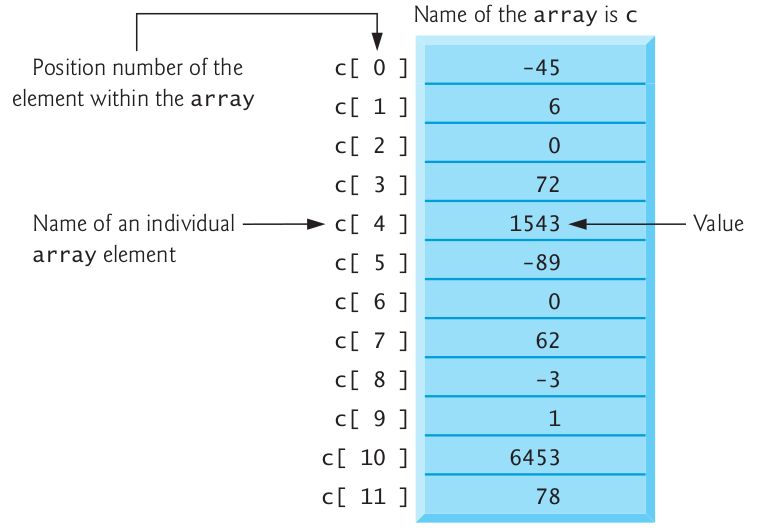
\includegraphics[width=8cm]{./.images/.img7-1.png}
	\end{center}
	
	A subscript must be an integer or integer expression (using any integral type). If a pro-
	gram uses an expression as a subscript, then the program evaluates the expression to deter-
	mine the subscript. For example, if we assume that variable a is equal to 5 and that variable
	b is equal to 6, then the statement
	
	\lstinputlisting[language=C++,firstline=1,lastline=1,numbers=none]{./.codes/.codes.cpp}
	
	
\end{frame}

\begin{frame}
	adds 2 to array element c[11]. A subscripted array name is an lvalue—it can be used on
	the left side of an assignment, just as non-array variable names can.
	Let’s examine array c in Fig. 7.1 more closely. The name of the entire array is c.
	Each array knows its own size, which can be determined by calling its size member func-
	tion as in c.size(). Its 12 elements are referred to as c[0] to c[11]. The value of c[0] is
	-45, the value of c[7] is 62 and the value of c[11] is 78. To print the sum of the values
	contained in the first three elements of array c, we’d write
	
	\lstinputlisting[language=C++,firstline=2,lastline=2,numbers=none]{./.codes/.codes.cpp}
	\\
	To divide the value of c[6] by 2 and assign the result to the variable x, we’d write
	\lstinputlisting[language=C++,firstline=3,lastline=3,numbers=none]{./.codes/.codes.cpp}
\end{frame}

\begin{frame}{\footnotesize Precedence and associativity of the operators introduced to this point}
	\centering\scriptsize\renewcommand{\arraystretch}{1.5}
	\begin{tabular}{p{0.5\linewidth} p{0.18\linewidth} p{0.18\linewidth}}
		
		\rowcolor{cyan}\color{white} Operator & \color{white} Associativity & \color{white} Type \\
		
		\rowcolor{lightcyan} \texttt{::} \hspace{2pt} \texttt{()} & left to right & primary \\
		\rowcolor{lightcyan} \texttt{()} \hspace{2pt} \texttt{[]} \hspace{2pt} \texttt{++} \hspace{2pt} \texttt{--} \hspace{2pt} \texttt{static\_cast<\textit{type}>(\textit{operand})} & left to right & postfix \\
		\rowcolor{lightcyan} \texttt{++} \hspace{2pt} \texttt{--} \hspace{2pt} \texttt{+} \hspace{2pt} \texttt{-} \hspace{2pt} \texttt{!} & right to left & prefix (unary) \\
		\rowcolor{lightcyan} \texttt{*} \hspace{2pt} \texttt{/} \hspace{2pt} \texttt{\%} & left to right & multiplicative \\
		\rowcolor{lightcyan} \texttt{+} \hspace{2pt} \texttt{-} & left to right & additive \\
		\rowcolor{lightcyan} \texttt{<<} \hspace{2pt} \texttt{>>} & left to right & insertion/extraction \\
		\rowcolor{lightcyan} \texttt{<} \hspace{2pt} \texttt{<=} \hspace{2pt} \texttt{>} \hspace{2pt} \texttt{>=} & left to right & relational \\
		\rowcolor{lightcyan} \texttt{==} \hspace{2pt} \texttt{!=} & left to right & equality \\
		\rowcolor{lightcyan} \texttt{\&\&} & left to right & logical AND \\
		\rowcolor{lightcyan} \texttt{||} & left to right & logical OR \\
		\rowcolor{lightcyan} \texttt{?:} & right to left & conditional \\
		\rowcolor{lightcyan} \texttt{=} \hspace{2pt} \texttt{+=} \hspace{2pt} \texttt{-=} \hspace{2pt} \texttt{*=} \hspace{2pt} \texttt{/=} \hspace{2pt} \texttt{\%=} & right to left & assignment \\
		\rowcolor{lightcyan} \texttt{,} & left to right & comma \\

	\end{tabular}
\end{frame}

\section{\texorpdfstring{Declaring \textbf{\textit{\color{lblue}arrays}}}{Declaring arrays}}
\begin{frame}{Declaring \textit{\color{blue}arrays}}
	arrays occupy space in memory. To specify the type of the elements and the number of
	elements required by an array use a declaration of the form \\
	\lstinputlisting[language=C++,firstline=4,lastline=4,numbers=none]{./.codes/.codes.cpp}
	The notation <type, arraySize> indicates that array is a class template. The compiler reserves
	the appropriate amount of memory based on the type of the elements and the arraySize.
	(Recall that a declaration which reserves memory is more specifically known as a defini-
	tion.) The arraySize must be an unsigned integer. To tell the compiler to reserve 12 ele-
	ments for integer array c, use the declaration
	\lstinputlisting[language=C++,firstline=5,lastline=5,numbers=none]{./.codes/.codes.cpp}
	arrays can be declared to contain values of most data types. For example, an array of type
	string can be used to store character strings.
\end{frame}

\section{\texorpdfstring{Examples Using \textbf{\textit{\color{lblue}arrays}}}{Examples Using arrays}}
\subsection{Declaring an array and Using a Loop to Initialize the array’s Elements}
\begin{frame}{\footnotesize Declaring an array and Using a Loop to Initialize the array’s Elements}
	The following examples demonstrate how to declare, initialize and manipulate arrays.\\
	
	\begin{block}{\color{white}Declaring an array and Using a Loop to Initialize the array’s Elements}
		The program in Fig. 7.3 declares five-element integer array n (line 9). Line 5 includes the
		<array> header, which contains the definition of class template array. Lines 12–14 use a
		for statement to initialize the array elements to zeros. Like other non-static local vari-
		ables, arrays are not implicitly initialized to zero (static arrays are). The first output
		statement (line 16) displays the column headings for the columns printed in the subse-
		quent for statement (lines 19–21), which prints the array in tabular format. Remember
		that setw specifies the field width in which only the next value is to be output.
	\end{block}
\end{frame}

\begin{frame}{}
	\lstinputlisting[language=C++]{../codes/chapter-7/example-7-1/example-7-1.cpp}
	\begin{block}{\color{white}output}
		\texttt{\scriptsize 
		Element\:\:\:Value\\
		\:\:\:\:\:\:\:\:\:\:\:\:\:\:0\:\:\:\:\:\:\:\:\:\:\:\:\:0\\
		\:\:\:\:\:\:\:\:\:\:\:\:\:\:1\:\:\:\:\:\:\:\:\:\:\:\:\:0\\
		\:\:\:\:\:\:\:\:\:\:\:\:\:\:2\:\:\:\:\:\:\:\:\:\:\:\:\:0\\
		\:\:\:\:\:\:\:\:\:\:\:\:\:\:3\:\:\:\:\:\:\:\:\:\:\:\:\:0\\
		\:\:\:\:\:\:\:\:\:\:\:\:\:\:4\:\:\:\:\:\:\:\:\:\:\:\:\:0\\}
	\end{block}
\end{frame}

\subsection{Initializing an array in a Declaration with an Initializer List}
\begin{frame}{\small Initializing an array in a Declaration with an Initializer List}
	\lstinputlisting[language=C++]{../codes/chapter-7/example-7-2/example-7-2.cpp}
	\begin{block}{\color{white}output}
		\texttt{\scriptsize 
			Element\:\:\:Value\\
			\:\:\:\:\:\:\:\:\:\:\:\:\:\:0\:\:\:\:\:\:\:\:\:\:32\\
			\:\:\:\:\:\:\:\:\:\:\:\:\:\:1\:\:\:\:\:\:\:\:\:\:27\\
			\:\:\:\:\:\:\:\:\:\:\:\:\:\:2\:\:\:\:\:\:\:\:\:\:64\\
			\:\:\:\:\:\:\:\:\:\:\:\:\:\:3\:\:\:\:\:\:\:\:\:\:18\\
			\:\:\:\:\:\:\:\:\:\:\:\:\:\:4\:\:\:\:\:\:\:\:\:\:95\\}
	\end{block}
\end{frame}

\subsection{Specifying an array’s Size with a Constant Variable}
\begin{frame}{\small Specifying an array’s Size with a Constant Variable}
	\small Example 7.3
	\lstinputlisting[language=C++]{../codes/chapter-7/example-7-3/example-7-3.cpp}
\end{frame}

\begin{frame}
	\begin{block}{\color{white}output}
		\texttt{\scriptsize 
			Element\:\:\:Value\\
			\:\:\:\:\:\:\:\:\:\:\:\:\:\:0\:\:\:\:\:\:\:\:\:\:\:\:2\\
			\:\:\:\:\:\:\:\:\:\:\:\:\:\:1\:\:\:\:\:\:\:\:\:\:\:\:4\\
			\:\:\:\:\:\:\:\:\:\:\:\:\:\:2\:\:\:\:\:\:\:\:\:\:\:\:6\\
			\:\:\:\:\:\:\:\:\:\:\:\:\:\:3\:\:\:\:\:\:\:\:\:\:\:\:8\\
			\:\:\:\:\:\:\:\:\:\:\:\:\:\:4\:\:\:\:\:\:\:\:\:\:10\\}
	\end{block}

	\begin{exampleblock}{Note}
		Line 8 uses the const qualifier to declare a {\color{purple}constant variable} \texttt{arraySize} with the value	5. Constant variables are also called \emph{\color{blue}named constants} or \emph{\color{blue}read-only} variables. A constant variable must be initialized when it’s declared and cannot be modified thereafter. Attempting to modify \texttt{arraySize} after it’s initialized, as in
		\lstinputlisting[language=C++,firstline=8,lastline=8,firstnumber=8]{../codes/chapter-7/example-7-3/example-7-3.cpp}
		
		\linebreak
		results in the following errors from Visual C++, GNU C++ and LLVM, respectively:
		\begin{itemize}
			\item Visual C++: \texttt{\footnotesize 'arraySize': you cannot assign to a variable that is const}
			\item GNU C++: \texttt{\footnotesize error: assignment of read-only variable ‘x’}
			\item LLVM: \texttt{\footnotesize Read-only variable is not assignable}
		\end{itemize}
	\end{exampleblock}
\end{frame}


\subsection{Summing the Elements of an array}
\begin{frame}{Summing the Elements of an array}
	Often, the elements of an array represent a series of values to be used in a calculation. For
	example, if the elements of an array represent exam grades, a professor may wish to total
	the elements of the array and use that sum to calculate the class average for the exam.
	The program in Fig. 7.6 sums the values contained in the four-element integer array
	a. The program declares, creates and initializes the array in line 9. The for statement
	(lines 13–15) performs the calculations. The values being supplied as initializers for array
	a also could be read into the program—for example, from the user at the keyboard or from
	a file on disk (see Chapter 14, File Processing). For example, the for statement
	\lstinputlisting[language=C++,firstline=6,lastline=9,numbers=none]{./.codes/.codes.cpp}
	reads one value at a time from the keyboard and stores the value in element \texttt{a[j]}.
\end{frame}
	
\begin{frame}
	\lstinputlisting[language=C++]{../codes/chapter-7/example-7-4/example-7-4.cpp}
	\begin{block}{\color{white}Output}
		\texttt{Total of array elements: 100}
	\end{block}
\end{frame}


\subsection{Using a Bar Chart to Display array Data Graphically}

\begin{frame}{Using a Bar Chart to Display array Data Graphically}
	\lstinputlisting[language=C++]{../codes/chapter-7/example-7-5/example-7-5.cpp}
\end{frame}

\begin{frame}
	\begin{block}{\color{white}Output}
		\texttt{Grade distribution:\\
		\:\:\:\:\:0-9:\\
		10-19:\\
		20-29:\\
		30-39:\\
		40-49:\\
		50-59:\\
		60-69: *\\
		70-79: **\\
		80-89: ****\\
		90-99: **\\
		\:\:\:\:\:100: *\\}
	\end{block}
\end{frame}


\subsection{Using the Elements of an array as Counters}
\begin{frame}{Using the Elements of an array as Counters}
	Sometimes, programs use counter variables to summarize data, such as the results of a sur-
	vey. In Fig. 6.7, we used separate counters in our die-rolling program to track the number
	of occurrences of each side of a die as the program rolled the die 60,000,000 times. An ar-
	ray version of this program is shown in Fig. 7.8. This version also uses the new C++11
	random-number generation capabilities that were introduced in Section 6.9.
	Figure 7.8 uses the array frequency (line 17) to count the occurrences of die value.
	The single statement in line 21 of this program replaces the entire switch statement in lines
	22–43 of Fig. 6.7. Line 21 uses a random value to determine which frequency element to increment during each iteration of the loop. The calculation in line 21 produces a random
	subscript from 1 to 6, so array frequency must be large enough to store six counters. We
	use a seven-element array in which we ignore frequency[0]—it’s clearer to have the die
	face value 1 increment frequency[1] than frequency[0]. Thus, each face value is used
	directly as a subscript for array frequency. We also replace lines 46–51 of Fig. 6.7 by
	looping through array frequency to output the results (Fig. 7.8, lines 27–29).
\end{frame}

\begin{frame}
	\lstinputlisting[language=C++]{../codes/chapter-7/example-7-6/example-7-6.cpp}
\end{frame}

\begin{frame}
	\begin{block}{\color{white}Output}
		\begin{tabular}{r r}
			Face & Frequency\\
			1 & 9997901\\
			2 & 9999110\\
			3 & 10001172\\
			4 & 10003619\\
			5 & 9997606\\
			6 & 10000592\\
		\end{tabular}
	\end{block}
increment during each iteration of the loop. The calculation in line 21 produces a random
subscript from 1 to 6, so array frequency must be large enough to store six counters. We
use a seven-element array in which we ignore frequency[0]—it’s clearer to have the die
face value 1 increment frequency[1] than frequency[0]. Thus, each face value is used
directly as a subscript for array frequency. We also replace lines 46–51 of Fig. 6.7 by
looping through array frequency to output the results (Fig. 7.8, lines 27–29).
\end{frame}

\subsection{Using arrays to Summarize Survey Results}
\begin{frame}{Using arrays to Summarize Survey Results}
	Our next example uses arrays to summarize the results of data collected in a survey. Con-
	sider the following problem statement:
	\begin{block}{Example}
		Twenty students were asked to rate on a scale of 1 to 5 the quality of the food in the
		student cafeteria, with 1 being “awful” and 5 being “excellent.” Place the 20 responses
		in an integer array and determine the frequency of each rating.
	\end{block}
This is a popular type of array-processing application (Fig. 7.9). We wish to summarize
the number of responses of each rating (that is, 1–5). The array responses (lines 14–15)
is a 20-element integer array of the students’ responses to the survey. The array respons-
es is declared const, as its values do not (and should not) change. We use a six-element
array frequency (line 18) to count the number of occurrences of each response. Each el-
ement of the array is used as a counter for one of the survey responses and is initialized to
zero. As in Fig. 7.8, we ignore frequency[0].
\end{frame}

\begin{frame}
	\lstinputlisting[language=C++]{../codes/chapter-7/example-7-7/example-7-7.cpp}
\end{frame}

\begin{frame}
	\begin{block}{\color{white}Output}
		\texttt{\begin{tabular}{r r}
			Rating & Frequency\\
			1 & 3\\
			2 & 5\\
			3 & 7\\
			4 & 2\\
			5 & 3\\
		\end{tabular}}
	\end{block}
\end{frame}

\subsection{Static Local arrays and Automatic Local arrays}
\begin{frame}{Static Local arrays and Automatic Local arrays}
	\lipsum[2]
\end{frame}

\begin{frame}
	\lstinputlisting[language=C++,lastline=31]{../codes/chapter-7/example-7-8/example-7-8.cpp}
\end{frame}
\begin{frame}
	\lstinputlisting[language=C++,firstline=32,firstnumber=32]{../codes/chapter-7/example-7-8/example-7-8.cpp}
\end{frame}
\begin{frame}
	\begin{block}{\color{white}Output}
		\texttt{\footnotesize
		First call to each function:
		\linebreak \linebreak
		Values on entering staticArrayInit:\\
		array1[0] = 0 array1[1] = 0 array1[2] = 0\\
		Values on exiting staticArrayInit:\\
		array1[0] = 5 array1[1] = 5 array1[2] = 5\\
		\linebreak 
		\vspace{8pt}
		\linebreak
		Values on entering automaticArrayInit:\\
		array2[0] = 1 array2[1] = 2 array2[2] = 3\\
		Values on exiting automaticArrayInit:\\
		array2[0] = 6 array2[1] = 7 array2[2] = 8\\
		\linebreak 
		\vspace{8pt}
		\linebreak
		Second call to each function:
		\linebreak 
		\linebreak
		Values on entering staticArrayInit:\\
		array1[0] = 5 array1[1] = 5 array1[2] = 5\\
		Values on exiting staticArrayInit:\\
		array1[0] = 10 array1[1] = 10 array1[2] = 10\\
		\linebreak 
		\vspace{8pt}
		\linebreak
		Values on entering automaticArrayInit:\\
		array2[0] = 1 array2[1] = 2 array2[2] = 3\\
		Values on exiting automaticArrayInit:\\
		array2[0] = 6 array2[1] = 7 array2[2] = 8}
	\end{block}
\end{frame}

\section{\texorpdfstring{Range-Based \textbf{\textit{\color{lblue}for}} Statement}{Range-Based for}}
\begin{frame}{Range-Based \textbf{\textit{\color{blue}for}} Statement}
	\lipsum[2]
\end{frame}

\section{Sorting and Searching}
\begin{frame}{Sorting and Searching}
	\lipsum[2]
\end{frame}

\section{\texorpdfstring{Multidimensional \textbf{\textit{\color{lblue}arrays}}}{Multidimensional array}}
\begin{frame}{Multidimensional \textbf{\textit{\color{blue}arrays}}}
	\lipsum[2]
\end{frame}

\section{\texorpdfstring{Introduction to C++ Standard Library Class Template \textbf{\textit{\color{lblue}vector}}}{Introduction to C++ Standard Library Class Template vector}}
\begin{frame}{Introduction to C++ Standard Library Class Template \textbf{\textit{\color{blue}vector}}}
	\lipsum[2]
\end{frame}

\section{Summery and Conclusion}

\begin{frame}{Summery and Conclusion}
	\lipsum[2]
\end{frame}


\section{Exercises}

\begin{frame}{Exercises}
	\lipsum[2]
\end{frame}

\begin{frame}{\small First Program in C++: Printing a Line of Text}
	
	Consider a simple program that prints a line of text (Fig. 2.1). This program illustrates several important features of the C++ language. The text in lines 1–10 is the program’s source code. The line numbers are not part of the source code.
	
	\lstinputlisting[language=C++]{../codes/chapter-2/fig_2-1/fig_2-1.cpp}
	
	\begin{block}{\textcolor{white}{output}}
		\texttt{\small Welcome to C++!}
	\end{block}
	
\end{frame}


\begin{frame}{\small The Stream Insertion Operator and Escape Sequences}
	\centering\tiny\renewcommand{\arraystretch}{2}	
\begin{tabular}{p{0.15\linewidth} p{0.6\linewidth}}
	\rowcolor{cyan}\color{white} Escape sequence & \color{white} Description \\
	
	\rowcolor{lightcyan} $\backslash$n & Newline. Position the screen cursor to the beginning of the next line.\\ 
	
	\rowcolor{lightcyan} $\backslash$t & Horizontal tab. Move the screen cursor to the next tab stop.\\ 
	
	\rowcolor{lightcyan} $\backslash$r & Carriage return. Position the screen cursor to the beginning of the current line; do not advance to the next line.\\ 
	
	\rowcolor{lightcyan} $\backslash$a & Alert. Sound the system bell.\\ 
	
	\rowcolor{lightcyan} $\backslash\backslash$ & Backslash. Used to print a backslash character.\\ 
	
	\rowcolor{lightcyan} $\backslash$' & Single quote. Used to print a single-quote character.\\ 
	
	\rowcolor{lightcyan} $\backslash$" & Double quote. Used to print a double-quote character.
\end{tabular}
\end{frame}


\begin{frame}{\small Arithmetic Operators}
	\centering\tiny\renewcommand{\arraystretch}{2}
	\begin{tabular}{p{0.15\linewidth} p{0.16\linewidth} p{0.2\linewidth} p{0.2\linewidth}}
		
		\rowcolor{cyan}\color{white} Operation & \color{white} Arithmetic operator & \color{white} Algebraic expression & \color{white} C++ expression \\
		
		\rowcolor{lightcyan} Addition & + & $f + 7$ & \texttt{f + 7} \\
		
		\rowcolor{lightcyan} Subtraction & - & $p - c$ & \texttt{p - c} \\
		
		\rowcolor{lightcyan} Multiplication & * & $bm$ or $b \cdot m$ & \texttt{b * m} \\
		
		\rowcolor{lightcyan} Division & / & $\dfrac{x}{y}$ or $x/y$ or $x\div y$ & \texttt{x / y} \\
		
		\rowcolor{lightcyan} Remainder & \% & $r$ $mod$ $s$ & \texttt{r \% s} 
	\end{tabular}
\end{frame}


\begin{frame}{\small Precedence of Arithmetic Operators}
	\centering\tiny\renewcommand{\arraystretch}{2}
	\begin{tabular}{p{0.12\linewidth} p{0.13\linewidth} p{0.65\linewidth}}
		
		\rowcolor{cyan}\color{white} Operator(s) & \color{white} Operation(s) & \color{white} Order of evaluation (precedence) \\\hline
		
		\rowcolor{lightcyan} \texttt{( )} & Parentheses & Evaluated first. For nested parentheses, such as in the expression
		\texttt{a * (b + c / (d + e))}, the expression in the innermost pair evalu ates first.\newline[Caution: If you have an expression such as \texttt{(a + b) * (c - d)} in which two sets of parentheses are not nested, but appear “on the same level,” the C++ Standard does not specify the order in which these parenthesized subexpressions will evaluate.] \\\hline
		
		\rowcolor{lightcyan} \texttt{*}\newline\texttt{/} \newline \texttt{\%} & Multiplication \newline Division \newline Remainder & Evaluated second. If there are several, they’re evaluated left to right. \\\hline
		
		\rowcolor{lightcyan} \texttt{+}\newline\texttt{-} & Addition \newline Subtraction & Evaluated last. If there are several, they’re evaluated left to right. \\\hline	
	\end{tabular}
\end{frame}



\begin{frame}{\small Decision Making: Equality and Relational Operators}
	\centering\tiny\renewcommand{\arraystretch}{2}
	\begin{tabular}{p{0.15\linewidth} p{0.15\linewidth} p{0.2\linewidth} p{0.25\linewidth}}
		
		\rowcolor{cyan}\color{white} Algebraic relational or equality operator & \color{white} C++ relational or equality operator & \color{white} Sample C++ condition & \color{white} Meaning of C++ condition \\\hline
		
		\rowcolor{lightcyan} \multicolumn{4}{l}{Relational operators} \\
		
		\rowcolor{lightcyan} $>$ & \texttt{>} & \texttt{x > y} & x is greater than y \\
		
		\rowcolor{lightcyan} $<$ & \texttt{<} & \texttt{x < y} & x is less than y \\
		
		\rowcolor{lightcyan} $\geq$ & \texttt{>=} & \texttt{x >= y} or & x is greater than or equal to y \\
		
		\rowcolor{lightcyan} $\leq$ & \texttt{<=} & \texttt{x <= y} & x is less than or equal to y \\\hline
		
		\rowcolor{lightcyan} \multicolumn{4}{l}{Equality operators} \\
		
		\rowcolor{lightcyan} $=$ & \texttt{==} & \texttt{x == y} & x is equal to y \\
		
		\rowcolor{lightcyan} $\neq$ & \texttt{!=} & \texttt{x != y} & x is not equal to y \\\hline
	\end{tabular}
\end{frame}


%
\end{document} 